\documentclass[tikz,crop]{standalone}

\usepackage{tikz}
\usetikzlibrary{arrows.meta,calc,shapes.geometric,positioning}

\definecolor{frontpanel color}{RGB}{236, 228, 226}
\definecolor{power button}{RGB}{253, 245, 243}
\definecolor{front-rear button}{RGB}{231, 219, 219}
\definecolor{bumper}{RGB}{155, 146, 151}
\definecolor{secondary button}{RGB}{77, 131, 157}
\definecolor{secondary label}{RGB}{142, 159, 179}
\definecolor{function button color}{RGB}{245, 238, 236}
\definecolor{option button color}{RGB}{211, 202, 205}
\definecolor{copper}{RGB}{183, 119, 41}

\begin{document}
    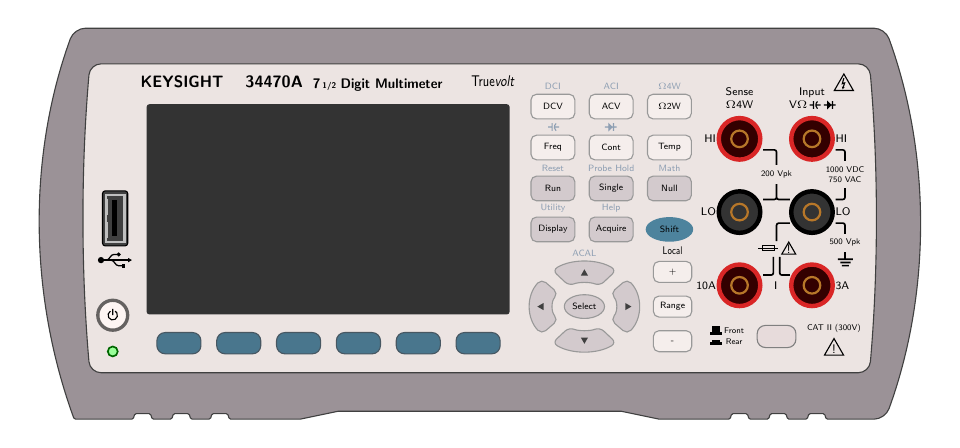
\begin{tikzpicture}[
        function button/.style={rectangle, minimum height=13.5, minimum width=24, font=\tiny, rounded corners=2, draw=black!40, fill=function button color, text centered, inner sep=0pt, scale=0.66, node font=\sffamily},
        screen button/.style={rounded corners=3, draw=cyan!30!black, fill=cyan!50!black},
        HI input/.style={circle, minimum size=15, draw=red!70!gray, line width=1.6pt, fill=red!20!black, inner sep=0pt},
        LO input/.style={circle, minimum size=15, draw=black, line width=1.6pt, fill=black!60!gray, inner sep=0pt},
        copper post/.style={circle, minimum size=6, draw=copper, line width=0.8pt, inner sep=0pt}
    ]
        \draw[darkgray, fill=bumper]
            [rounded corners] (-5.1,-2.5) arc(200:160:22.5/3.1) -- ++(10.3,0) arc(20:-20:22.5/3.1) [rounded corners=0.5] -- ++(-0.75,0) -- ++(-0.02,0.07) -- ++(-0.2,0) -- ++(-0.02,-0.07) -- ++(-0.25,0) -- ++(-0.02,0.07) -- ++(-0.2,0) -- ++(-0.02,-0.07) -- ++(-0.25,0) -- ++(-0.02,0.07) -- ++(-0.2,0) -- ++(-0.02,-0.07) [sharp corners] -- ++(-0.9,0) -- ++(-0.48,0.1)
            -- ++(-3.6,0)
            -- ++(-0.48,-0.1) [rounded corners=0.5] -- ++(-0.9,0) -- ++(-0.02,0.07) -- ++(-0.2,0) -- ++(-0.02,-0.07) -- ++(-0.25,0) -- ++(-0.02,0.07) -- ++(-0.2,0) -- ++(-0.02,-0.07) -- ++(-0.25,0) -- ++(-0.02,0.07) -- ++(-0.2,0) -- ++(-0.02,-0.07) -- cycle
        ;
        % front panel
        \begin{scope}
            \draw[darkgray, fill=frontpanel color, rounded corners]
                (-4.9,-1.91) arc(185:175:22.5) -- ++(9.9,0) arc(5:-5:22.5) -- cycle
            ;
            \node[yscale=0.85, xscale=0.8, font=\scriptsize, node font=\sffamily\bfseries] at (-3.73,1.78) {KEYSIGHT};
            \node[scale=0.85, font=\scriptsize, node font=\sffamily\bfseries] at (-2.56,1.78) {34470A};
            \node[font=\tiny, node font=\sffamily\bfseries] at (-2.02,1.76) {7};
            \node[scale=0.6, font=\tiny, node font=\sffamily\bfseries] at (-1.86,1.72) {1/2};
            \node[xscale=0.95, font=\tiny, node font=\sffamily\bfseries] at (-1.07,1.74) {Digit Multimeter};
            \node[xscale=0.6, yscale=0.8, font=\scriptsize, node font=\sffamily] at (0.22,1.79) {True\textit{volt}};
        \end{scope}
        % screen
        \begin{scope}
            \fill[rounded corners=1, black!80] (-4.18,-1.17) rectangle (0.43,1.5);
            % bottom row buttons
            \foreach \x in {0,...,5} {
                \fill[screen button] (-4.05+\x*0.76,-1.67) rectangle ++(0.56,0.27);
            }
        \end{scope}  % screen
        % function buttons
        \begin{scope}[]
            % 1st row
            \node[function button] at (0.98,1.47) {DCV};
            \node[above=1.3mm, font=\tiny, node font=\sffamily, text=secondary label, scale=0.66] at (0.98,1.47) {DCI};
            \node[function button] at (1.72,1.47) {ACV};
            \node[above=1.3mm, font=\tiny, node font=\sffamily, text=secondary label, scale=0.66] at (1.72,1.47) {ACI};
            \node[function button] at (2.46,1.47) {$\Omega$2W};
            \node[above=1.3mm, font=\tiny, node font=\sffamily, text=secondary label, scale=0.66] at (2.46,1.47) {$\Omega$4W};
            % 2nd row
            \node[function button] at (0.98,0.95) {Freq};
            \draw[secondary label]
                (0.92,1.21) -- ++(0.05,0) ++(0,0.05) -- ++(0,-0.1) ++(0.03,0.05) -- ++(0.06,0) ++(-0.04,0.045) arc (130:230:0.06)
            ;
            \node[function button] at (1.72,0.95) {Cont};
            \draw[fill, secondary label]
                (1.64,1.21) -- ++(0.05,0) -- ++(0,0.04) -- ++(0.04,-0.04) -- ++(-0.04,-0.04) -- ++(0,0.04) ++(0.04,0) -- ++(0.06,0) ++ (-0.04,0.05) -- ++(0,-0.1)
            ;
            \node[function button] at (2.46,0.95) {Temp};
            % 3rd row
            \node[function button, fill=option button color] at (0.98,0.43) {Run};
            \node[above=1.3mm, font=\tiny, node font=\sffamily, text=secondary label, scale=0.66] at (0.98,0.43) {Reset};
            \node[function button, fill=option button color] at (1.72,0.43) {Single};
            \node[above=1.3mm, font=\tiny, node font=\sffamily, text=secondary label, scale=0.66] at (1.72,0.43) {Probe Hold};
            \node[function button, fill=option button color] at (2.46,0.43) {Null};
            \node[above=1.3mm, font=\tiny, node font=\sffamily, text=secondary label, scale=0.66] at (2.46,0.43) {Math};
            % 4th row
            \node[function button, fill=option button color] at (0.98,-0.09) {Display};
            \node[above=1.3mm, font=\tiny, node font=\sffamily, text=secondary label, scale=0.66] at (0.98,-0.09) {Utility};
            \node[function button, fill=option button color] at (1.72,-0.09) {Acquire};
            \node[above=1.3mm, font=\tiny, node font=\sffamily, text=secondary label, scale=0.66] at (1.72,-0.09) {Help};
            \node[ellipse, minimum height=13.5, minimum width=26, font=\tiny, fill=secondary button, text centered, inner sep=0pt, scale=0.66, node font=\sffamily] at (2.46,-0.09) {Shift};
            \node[function button, minimum height=11.5, minimum width=21] at (2.5,-0.63) {+};
            \node[yscale=0.8, xscale=0.6, above=1mm, font=\tiny, node font=\sffamily] at (2.5,-0.61) {Local};
            \node[function button, minimum height=11.5, minimum width=21] at (2.5,-1.07) {Range};
            \node[function button, minimum height=11.5, minimum width=21] at (2.5,-1.51) {-};

            % Navigation keys
            \begin{scope}[shift={(1.38,-1.07)}]
            \node[ellipse, minimum height=13, minimum width=22, font=\tiny, draw=black!40, fill=option button color, text centered, inner sep=0pt, scale=0.66, node font=\sffamily] at (0,0) {Select};
                \draw[black!40, fill=option button color, rounded corners=2]  (126:0.69 and 0.57) arc (126:54:0.69 and 0.57)
                    -- (61:0.4 and 0.3) arc (61:119:0.4 and 0.3)
                    -- cycle;
                \node[regular polygon, regular polygon sides=3, fill=darkgray, minimum size=3, inner sep=0pt] at (0,0.42) {};
                \node[above=1.3mm, font=\tiny, node font=\sffamily, text=secondary label, scale=0.66] at (0,0.42) {ACAL};
                \draw[black!40, fill=option button color, rounded corners=2]  (-126:0.69 and 0.57) arc (-126:-54:0.69 and 0.57)
                    -- (-61:0.4 and 0.3) arc (-61:-119:0.4 and 0.3)
                    -- cycle;
                \node[regular polygon, regular polygon sides=3, fill=darkgray, minimum size=3, inner sep=0pt, rotate=180] at (0,-0.42) {};
                \draw[black!40, fill=option button color, rounded corners=2]  (38:0.69 and 0.57) arc (38:-38:0.69 and 0.57)
                    -- (-34:0.4 and 0.3) arc (-34:34:0.4 and 0.3)
                    -- cycle;
                \node[regular polygon, regular polygon sides=3, fill=darkgray, minimum size=3, inner sep=0pt, rotate=-90] at (0.545,0) {};
                \draw[black!40, fill=option button color, rounded corners=2]  (218:0.69 and 0.57) arc (218:142:0.69 and 0.57)
                    -- (146:0.4 and 0.3) arc (146:214:0.4 and 0.3)
                    -- cycle;
                \node[regular polygon, regular polygon sides=3, fill=darkgray, minimum size=3, inner sep=0pt, rotate=90] at (-0.545,0) {};
            \end{scope}
        \end{scope} % function buttons

        % input terminals
        \begin{scope}[]
            % 1st row
            \node[HI input] (input HI sense) at (3.35,1.06) {};
            \node[copper post] at (input HI sense) {};
            \node[left=2mm, font=\tiny, node font=\sffamily, scale=0.8] at (input HI sense) {HI};
            \node[above=2.8mm, font=\tiny, node font=\sffamily, align=center, scale=0.8] at (input HI sense) {Sense\\$\Omega$4W};
            \node[HI input] (input HI) at (4.27,1.06) {};
            \node[copper post] at (input HI) {};
            \node[right=2mm, font=\tiny, node font=\sffamily, scale=0.8] at (input HI) {HI};
            \node[above=2.8mm, font=\tiny, node font=\sffamily, align=center, scale=0.8] at (input HI) {Input\\V$\Omega$\ \ \ \ \ \ \ \ };
            % capacitor
            \draw
                (4.24,1.49) -- ++(0.05,0) ++(0,0.05) -- ++(0,-0.1) ++(0.03,0.05) -- ++(0.06,0) ++(-0.04,0.045) arc (130:230:0.06)
            ;
            % diode
            \draw[fill]
                (4.42,1.49) -- ++(0.05,0) -- ++(0,0.04) -- ++(0.04,-0.04) -- ++(-0.04,-0.04) -- ++(0,0.04) ++(0.04,0) -- ++(0.06,0) ++ (-0.04,0.05) -- ++(0,-0.1)
            ;
            % 2nd row
            \node[LO input] (input LO sense) at (3.35,0.13) {};
            \node[copper post] at (input LO sense) {};
            \node[left=2mm, font=\tiny, node font=\sffamily, scale=0.8] at (input LO sense) {LO};
            \node[LO input] (input LO) at (4.27,0.13) {};
            \node[copper post] at (input LO) {};
            \node[right=2mm, font=\tiny, node font=\sffamily, scale=0.8] at (input LO) {LO};
            % 3rd row
            \node[HI input] (input current 10A) at (3.35,-0.8)  {};
            \node[copper post] at (input current 10A) {};
            \node[left=2mm, font=\tiny, node font=\sffamily, scale=0.8] at (input current 10A) {10A};
            \node[HI input] (input current 3A) at (4.27,-0.8) {};
            \node[copper post] at (input current 3A) {};
            \node[right=2mm, font=\tiny, node font=\sffamily, scale=0.8] at (input current 3A) {3A};
            \node[font=\tiny, node font=\sffamily, scale=0.8] at ($(input current 10A)!0.5!(input current 3A)$) {I};
            % Input terminals connection drawing
            \draw[rounded corners=0.8, line width=0.6]
                (3.65,0.92) -- ++(0.17,0) -- ++(0,-0.63) -- ++(-0.17,0)
                (3.82, 0.4) -- ++(0,-0.11) -- ++(0.17,0)
            ;
            \node[font=\tiny, node font=\sffamily, scale=0.6, fill=frontpanel color] at ($(3.82, 0.92)!0.5!(3.82,0.29)$) {200 Vpk};
            \draw[rounded corners=0.8, line width=0.6]
                (4.57,0.92) -- ++(0.12,0) -- ++(0,-0.63) -- ++(-0.12,0)
            ;
            \node[font=\tiny, node font=\sffamily, align=center, scale=0.6, fill=frontpanel color] at ($(4.69, 0.92)!0.5!(4.69,0.29)$) {1000 VDC\\750 VAC};
            \draw[rounded corners=0.8, line width=0.6]
                (4.57,-0.01) -- ++(0.12,0) -- ++(0,-0.46)
                (4.6,-0.47) -- ++(0.19,0)
                (4.63,-0.51) -- ++(0.13,0)
                (4.65,-0.55) -- ++(0.09,0)
            ;
            \node[font=\tiny, node font=\sffamily, align=center, scale=0.6, fill=frontpanel color] at ($(4.69, -0.01)!0.5!(4.69,-0.51)$) {500 Vpk};
            \draw[rounded corners=0.8, line width=0.6]
                (3.99,-0.01) -- ++(-0.17,0) -- ++(0,-0.23)
                (3.78,-0.44) -- ++(0,-0.23) -- ++(-0.13,0)
                (3.86,-0.44) -- ++(0,-0.23) -- ++(0.13,0)
            ;
            % fuse
            \draw
                (3.59,-0.33) -- ++(0.25,0)
                ++(-0.20,0.03) -- ++(0.15,0) -- ++(0,-0.06) -- ++(-0.15,0) -- cycle
                node[right=3.35mm, yshift=-1.8, isosceles triangle, isosceles triangle apex angle=60, draw, rotate=90, scale=0.35, anchor=center] (fuse warning) {}
                node[yshift=0.5, font=\tiny, node font=\sffamily, scale=0.9] at (fuse warning) {!}
            ;
            % high voltage warning
            \draw
                (4.675,1.73)
                node[isosceles triangle, isosceles triangle apex angle=60, draw, rotate=90, scale=0.48] (high voltage) {}
                (high voltage.apex) ++(0,-0.06) -- ++(-0.02,-0.07) -- ++(0.03,0.01) -- ++(-0.02,-0.06)
                node[isosceles triangle, fill, isosceles triangle apex angle=60, scale=0.07, rotate=-108.4] {}
            ;
        \end{scope}  % input terminals
        % CAT Rating
        \draw
            (4.55,-1.63)
            node[isosceles triangle, isosceles triangle apex angle=60, draw, rotate=90, scale=0.48] (CAT rating) {}
            node[yshift=0.5, font=\tiny, node font=\sffamily, scale=0.9] {!}
            node[above=0.15, font=\tiny, node font=\sffamily, scale=0.6] at (CAT rating) {CAT II (300V)}
        ;
        % USB port
        \begin{scope}
            \draw[rounded corners=1, fill=darkgray]
                (-4.74,0.4) -- ++(0.32,0) -- ++(0,-0.7) -- ++(-0.32,0) -- cycle
            ;
            \draw[lightgray, fill=darkgray, line width=0.8pt]
                (-4.7,0.35) -- ++(0.24,0) -- ++(0,-0.6) -- ++(-0.24,0) -- cycle
                (-4.68,0.3) -- ++(0,-0.21)
                (-4.68,-0.2) -- ++(0,0.21)
            ;
            \draw[line width=1.6pt]
                (-4.59,0.28) -- ++(0,-0.46)
            ;
            % USB symbol
            \pgfmathsetmacro\scl{0.04}  %scaling factor of the usb symbol
            \begin{scope}[scale=\scl]
                \node [circle, minimum size=\scl*20mm, fill, inner sep=0pt] (start) at (-4.76/\scl,-0.48/\scl) {};
                \draw[line width=\scl*4mm, arrows = {-Stealth[scale=\scl, inset=0pt, length=12.3mm, angle'=55]}]
                    (start.center) -- ++(9.82,0)
                ;
                \draw[line width=\scl*4mm, arrows = {-Circle[scale=\scl, length=12mm]}]
                    (start.center) -- ++(1.6,0) to[out=0, in=234.2461] ++(1.25,0.9) to[out=54.2461, in=180] ++(1.25,0.9) -- ++(2.1,0)
                ;
                \draw[line width=\scl*4mm, arrows = {-Square[scale=\scl, length=12mm]}]
                    (start.center) -- ++(3.1,0) to[out=0, in=-234.2461] ++(1.25,-0.9) to[out=-54.2461, in=180] ++(1.25,-0.9) -- ++(2.1,0)
                ;
            \end{scope}
        \end{scope}
        % power button amd led
        \begin{scope}
            \node [circle, minimum size=10.8, draw=power button!40!black, line width=1.2pt, fill=power button, inner sep=0pt] at (-4.61,-1.18) {};
            \draw
                ($(-4.61,-1.18) + (120:0.06)$) arc (120:420:0.06)
                (-4.61,-1.1) -- ++(0,-0.08)

            ;
            % power led
            \node[circle, minimum size=6, draw=green!40!black, line width=0.6pt, fill=green!40, inner sep=0pt, scale=0.6] at (-4.61,-1.64) {};

        \end{scope}  % power button
        % front/rear button
        \begin{scope}
            \draw[fill]
                (2.98,-1.42) -- ++(0,0.02) -- ++(0.03,0) -- ++(0,0.08) -- ++(0.08,0) -- ++(0,-0.08) -- ++(0.03,0) -- ++(0,-0.02) -- ++(-0.14,0) -- cycle
                node[right=0.1, yshift=1.4, font=\tiny, node font=\sffamily, scale=0.6] (Front label) {Front}
            ;

            \draw[fill]
                (2.98,-1.55) -- ++(0,0.02) -- ++(0.03,0) -- ++(0,0.03) -- ++(0.08,0) -- ++(0,-0.03) -- ++(0.03,0) -- ++(0,-0.02) -- ++(-0.14,0) -- cycle
                node[below=-0.08 of Front label, font=\tiny, node font=\sffamily, scale=0.6] {Rear}
            ;
            \node[rectangle, minimum height=8, minimum width=14, rounded corners=3, draw=black!50, fill=front-rear button, text centered, inner sep=0pt] at (3.82,-1.45) {};
        \end{scope}
    \end{tikzpicture}
\end{document}
